\section{Comparing Candidate Elements to the Nearest Asteroid}
Before we review the results of our asteroid search experiments, it will be helpful to have in hand a notion of how closely two sets of orbital elements match.
In particular, we will test below whether or not we successfully recovered orbital elements when we started with them as an initial guess.
Answering this question requires that we have a useful metric on the space of orbital elements.

I spent a fair amoutn of time trying to develop such a metric.
While orbital elements are convenient for intuition and calculating orbits, there isn't an obvious distance metric we can put on them that makes a lot of sense.
Eventually I decided that the canonical way to compare two orbits by comparing the predicted vector of positions on a set of representative dates.
Logically this is hard to argue with, but it is somewhat computationally expensive compared to a computation that can be run directly on the elements.

The method \tty{nearest\_ast} searches the asteroid catalogue for the known asteroid whose orbit is closest to that predicted by the candidate elements.
It delegates its work to the function \tty{nearest\_ast\_elt\_cart}, which is defined in \tty{nearest\_asteroid.py}.
This function creates a set of 240 sample time points over 20 years spanning 2010 to 2030 sampled monthly.
The resulting table of positions for the asteroid catalog is fairly large, with a size of $[733490, 240, 3]$ (5.28E8 elements and about 2.11 GB using 32 bit floats).
Computing the nearest asteroid against $64$ candidate elements by brute force in TensorFlow would necessitate creating a tensor with 3.38E10 elements
or 135 GB of memory--two orders of magnitude too large for a high quality consumer grade GPU with $\sim 10$ GB of memory.
The nearest asteroid method is therefore forced to iterate through the elements one at a time, taking the norm of the difference against the table.
In one important optimization, the tensor of known asteroid positions in loaded into memory 
once as a TensorFlow constant to avoid recomputing it every time the function is called.

I also sought to develop a sensible metric of the distance between a pair of arbitrary orbital elements.
This is implemenented in the same module with the function \tty{elt\_q\_norm} and \tty{nearest\_ast\_elt\_cov}.
The idea is to transform the elements to a Cartesian representation where they have a well behaved covariance matrix.
In particular, the goal is to find a deterministic transform of the elements that is distributed approximately as a multivariate normal.
Then the \href{https://en.wikipedia.org/wiki/Mahalanobis_distance}{Mahalanobis distance} is a natural metric on the transformed elements.
This process can be reviewed in the Jupyter notebook \tty{11\_nearest\_asteroid.ipynb}.
I initially tried working with the full empirical distribution to convert every orbital element to a percentile and then to a normally distributed $z$ score,
but the results didn't make any sense, so I dropped that approach.

Instead, I switched to a simpler approach and standardized variables so they would have mean zero and variance 1.
I attempt to make them close to normal if possible, but without overfitting against the empirical distribution.
I standardized the log of the semimajor axis $a$ and directly standardized the eccentricity $e$.
(Even though this admits mappings from $z$ to eccentirities outside $[0,1]$, the mapping is only used in the direction
from a reported eccentricity $e$ to a transformed $e_z$ that is approximately normal).
The quantity $\sin(inc)$ was also also standardized.
Here is a summary of the mathematical transformations to create approximately normal variables from $a$, $e$ and $i$:
\begin{align*}
a_z &= \frac{\log(a) - \E[\log(a)]}{\sqrt{\Var[\log(a)]}} \\
e_z &= \frac{e - \E[e]}{\sqrt{\Var[e]}} \\
i_z &= \frac{\sin(i) - \E[\sin(i)]}{\sqrt{\Var[\sin(i)]}}
\end{align*}
The expectation and variance here are estimated using the sample mean and sample variance respectively.

Here are visualizations of comparing the hypothetical and empirical distributions of $a$ and $e$:
\begin{figure}[hbt!]
\begin{center}
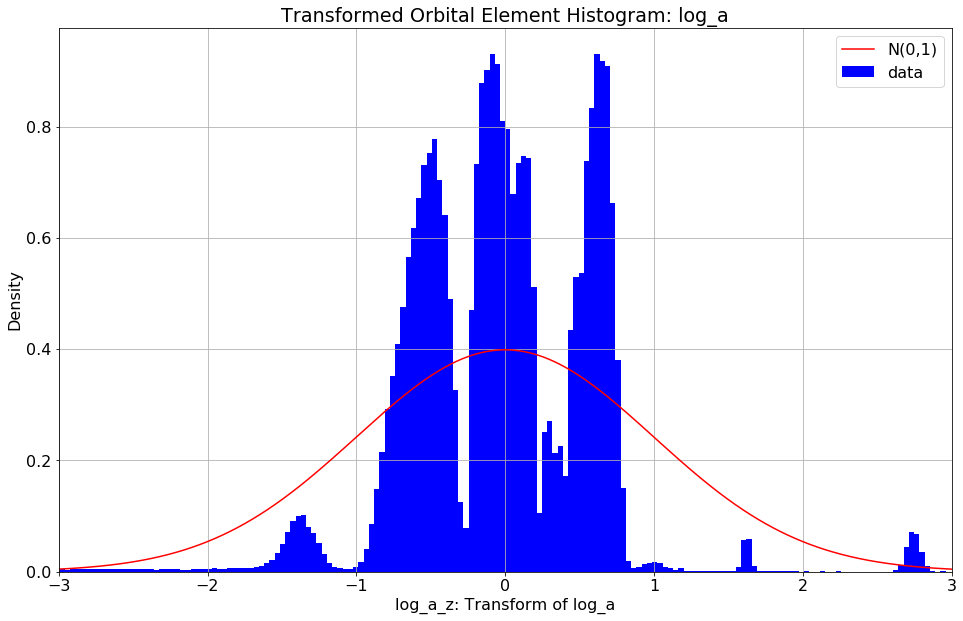
\includegraphics[width=0.8\textwidth]{../figs/elts_cov/log_a_z.png}
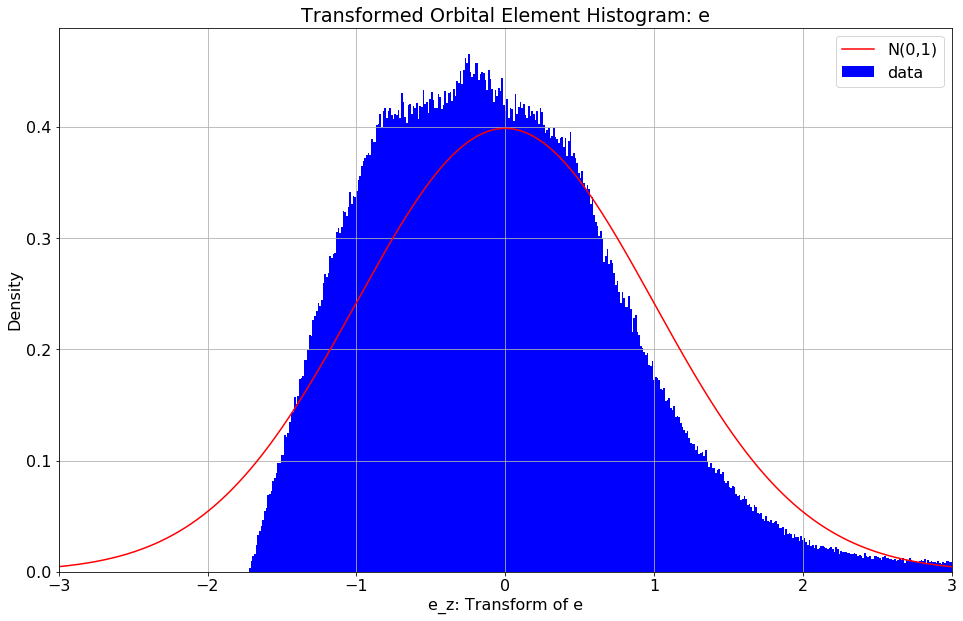
\includegraphics[width=0.8\textwidth]{../figs/elts_cov/e_z.png}
\caption{Transformations of $a$ and $e$ to standardized (and ``approximately'' normal) variables $a_z$ and $e_z$.}
\end{center}
\end{figure}
\clearpage

The other three angular orbital elements $\Omega$, $\omega$ and $f$ are handled identically.
We can inject $i$ into Cartesian space with only its sine because it is constrained to $[-\pi, \pi]$.
But the other three angles are unconstrained.  I will take $\Omega$ as an example.
I transform $\Omega$ into \textit{two} variables, named \tty{cos\_Omega\_z} and \tty{sin\_Omega\_z}.
These are not transformed empirically, but using a theoretical distribution.
Let $x$ be the sine or cosine of one of $\Omega$, $\omega$ or $f$.
$x$ is mapped to a variable $z$ that is distributed appproximately normal by applying the tranformation
\begin{align*}
u &= \frac{1/2 + \arcsin(x)}{\pi} \\
z &= \Phi^{-1}(u)
\end{align*}
where $\Phi$ is normal CDF.

Below are visualizations of comparing the hypothetical and empirical distributions of $\sin(i)$ and $\sin(\Omega)$:
\begin{figure}[hbt!]
\begin{center}
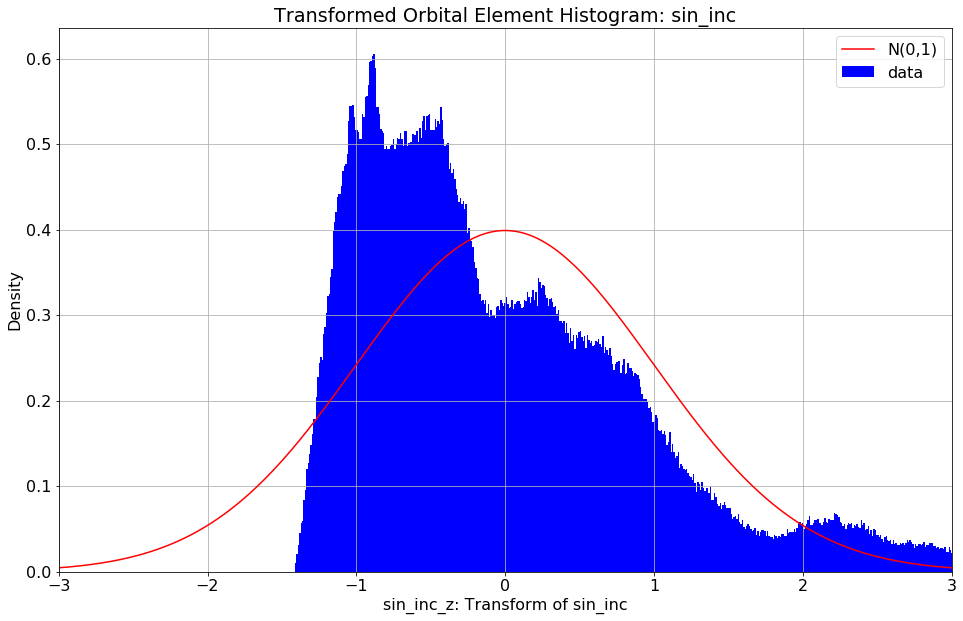
\includegraphics[width=0.8\textwidth]{../figs/elts_cov/sin_inc_z.png}
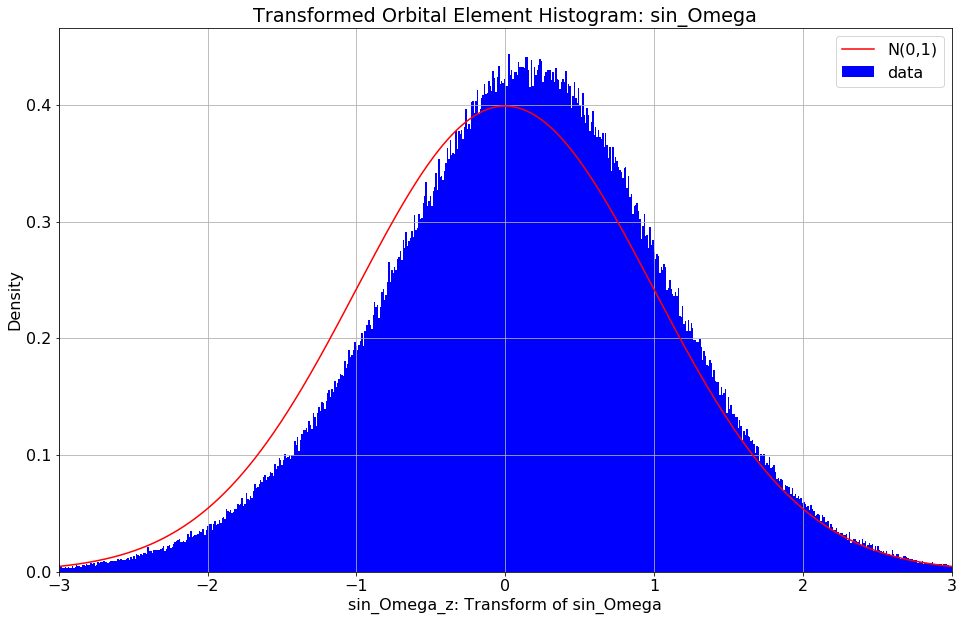
\includegraphics[width=0.8\textwidth]{../figs/elts_cov/sin_Omega_z.png}
\caption{Transformations of $a$ and $e$ to standardized (and ``approximately'' normal) variables $a_z$ and $e_z$.}
\end{center}
\end{figure}

Better results for $e$ and $i$ could be obtained by using the Beta distributions noted above, for this purpose the simple standardization is adequate.
The plot shown for the tranform of $\sin(\Omega)$ shows that it is very close to the theoretical distribution.
I generated analogous plots for the $\sin$ and $\cos$ of $\Omega$, $\omega$ and $f$ which are in the Jupyter notebook.
They are qualitatively similar to this one and all show excellent fits.

I have now given a recipe with which six orbital elements can be injected into $R^{9}$.
Let $X$ be the $N x 9$ matrix of transformed elements ($N$ = 733,489 is the number of asteroids).
The orbital elements are only very lightly correlated with each other, 
and so are the $X_j$ except for the tightly correlated pairs with the $\sin$ and $\cos$ of the same angle.
Next, using the Spectral Theorem, I find a $9x9$ matrix $\beta$ such that the covariance matrix of $X \beta$  
(which also has shape $N x 9$) is the $9x9$ identity matrix.
The only wrinkle is that I assign importance weights to the 9 columns before building $X$ and computing $\beta$.
The importance weights are:
\begin{itemize}
\item 1.0 for $a_z$ and $e_z$
\item 0.5 for $i_z$
\item 0.1 for the $\sin$ and $\cos$ of $\Omega$, $\omega$ and $f$
\end{itemize}
These are admittedly qualitiative judgments on my part. 
I initially only compensated for the double counting of $\Omega$, $\omega$ and $f$, 
but I noticed that relatively small differences in e.g. $\omega$ on a near circular orbit that hardly effected the shape of an orbit
were having a disproportionately large influence of covariance score.

The covariance metric between two sets of orbital elements is $\epsilon_1$ and $\epsilon_2$ is defined by
$$ \norm{\epsilon_2 - \epsilon_1}_{\mathrm{cov}} = \norm{\epsilon_2 \beta - \epsilon_1 \beta} $$
The importance weights are rescaled so the diagonal of the covariance matrix sums to $1$ and a random pair of elements should have distance 1.
These calculations are also in \tty{nearest\_asteroid.py} and done by the 
functions \tty{elts\_to\_X\_cov}, \tty{calc\_beta}, \tty{elt\_q\_norm} and \tty{nearest\_ast\_elt\_cov}.
Now that we know what it means for two orbital elements to be ``close,'' 
we are ready for our first test: recovering unperturbed elements.

\section{Recovering the Unperturbed Elements of Known Asteroids}
\label{section_results_known_ast_unperturbed}

The first and easiest proof of concept for the search process is to see if the mixture parameters will converge correctly
when the search is initialized with correct orbital elements for asteroids that are well represented in the data,
but with ``neutral'' or uninformative mixture parameters.
I liken this test to a kid learning to swing a bat by trying to ball sitting on a tee.
This test is demonstrated in the Jupyter notebook \tty{14\_asteroid\_search\_unperturbed.ipynb}.
It was developed before the automated sieving routine, so it includes lower level calls to the \tty{adaptive\_search} method.

It's worthwhile to follow through the steps to assemble the data to get familiar with how everything fits together.
These two lines of codes load the ZTF data observations associated with the nearest asteroid, and count hits by asteroid number:
\begin{lstlisting}[style=CodeSnippet]
ast_elt = load_ztf_nearest_ast()
ast_num, hit_count = calc_hit_freq(ztf=atf_ast, thresh_Sec=2.0)
\end{lstlisting}
The next few lines sort the asteroids in descending order by number of hits, 
and assemble a data frame of the orbital elements belonging to the 64 ``best'' asteroids
The function \tty{asteroid\_elts} in \tty{candidate\_elements} provides a batch of candidate orbital elements
that exactly match known asteroids; it assigns an \tty{element\_id} matching the original asteroid number to make it easy
to check later if the fitted elements match the original.
The function \tty{load\_ztf\_batch} assembles the batch of ZTF observations within a threshold, 
here 2.0 degrees, of these candidate elements
\begin{lstlisting}[style=CodeSnippet]
elts_ast = asteroid_elts(ast_nums=ast_num_best[0:64])
ztf_elt = load_ztf_batch(elts=elts_ast, thresh_deg=2.0)
\end{lstlisting}

Reviewing the \tty{ztf\_elt} on screen we can see that there are 322,914 rows which include 10,333 hits:
an averate of 161.5 hits per candidate element and 3.2\% of the total rows of data.
A call to \tty{score\_by\_elt} computes the t-score described earlier based on the mean and standard deviation of $\log(v)$.
This shows a mean t-score of +45.0, which is off the charts good.
It's interesting to see that a set of observations with 3.2\% hits and 96.8\% noise achieves such a good score.
This also puts into context the challenge of the search problem: 
we have an average of 5045 detections within 2.0 degrees of each set of candidate elements,
of which 160 are hits and the remaining 4885 are random detections belonging to other asteroids.
If we want a search process to detect asteroids with as few as 8 hits in the data, 
we will need a process selective enough to pick out just 0.16\% of the observations.

To initiate the search, we also need to choose our initial mixture parameters.
we set \tty{num\_hits} to $10$ and the resolution to $0.5$ degrees
\begin{lstlisting}[style=CodeSnippet]
elts_add_mixture_params(
	elts=elts, num_hits=num_hits, 
	R_deg=R_deg, thresh_deg=thresh_deg)
\end{lstlisting}

Now that we have the candidate elements and the ZTF data frame, we are ready to instantiate the asteroid search model:
\begin{lstlisting}[style=CodeSnippet]
model = AsteroidSearchModel(
	elts=elts_ast, ztf_elt=ztf_elt, 
	site_name='palomar', thresh_deg=2.0)
\end{lstlisting}
Before we start training the model, we can get a plain text report or a visualization of the starting point.
I will omit these here. 
The report shows that at the start of training, 10 elements are ``good'' with 5 or more hits,
and the overall mean log likelihood is 3.13 and the mean number of hits is 3.19.
\footnote{
As I write this, I realize that something is going wrong somewhere.
The initial model should show the same number of hits, 10,333, as the ZTF data frame.
There must be some slippage between the CPU / \tty{numpy} calculations and the TensorFlow GPU model
on the order of 10 arc seconds or more to explain this.  I will investigate this later.}

\begin{minipage}{\linewidth}
Here is an excerpt from the plain text model report:
\begin{lstlisting}[style=CodeSnippet]
model.report()

Good elements (hits >= 5):  64.00
         \  log_like :  hits  :    R_sec : thresh_sec
Mean Good:  1057.30  : 136.75 :     7.05 :   347.11
Mean Bad :      nan  :    nan :      nan :      nan
Min      :   848.14  :  15.00 :     1.97 :   112.80
Max      :  1307.20  : 190.00 :    14.87 :   697.68
Trained for 9536 batches over 149 epochs and 59 episodes (elapsed time 425 seconds). 
\end{lstlisting}
\end{minipage}

I've developed a number of visualizations to assess training progress.
\newcommand{\subfigwidth}{0.5}
\begin{figure}[h]
\begin{subfigure}[t]{\subfigwidth\textwidth}
\centering
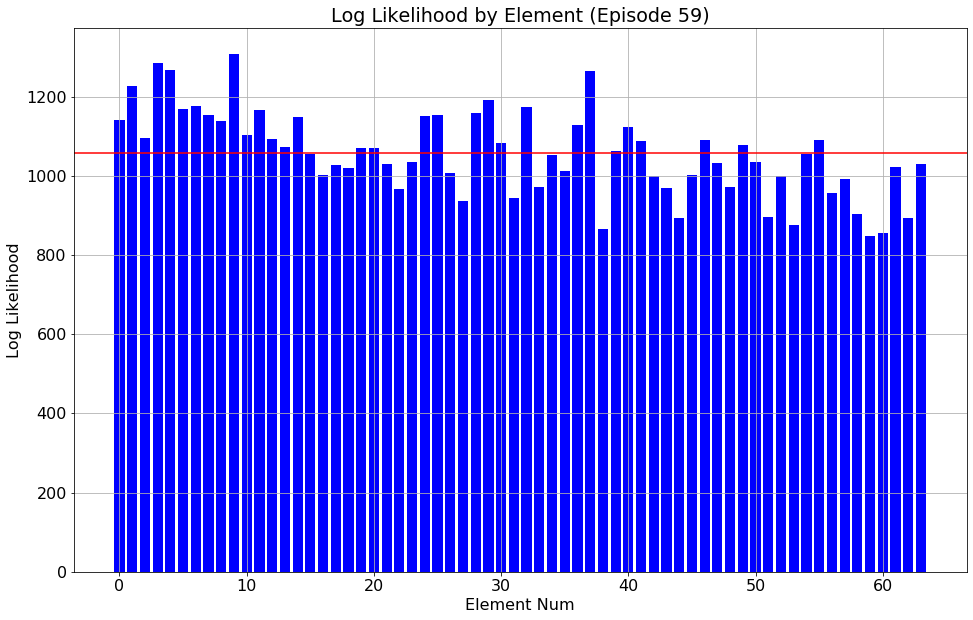
\includegraphics[width=\linewidth]{../figs/search_known/unperturbed/log_like.png}
% \caption{}
\end{subfigure}
\hfill
\begin{subfigure}[t]{\subfigwidth\textwidth}
\centering
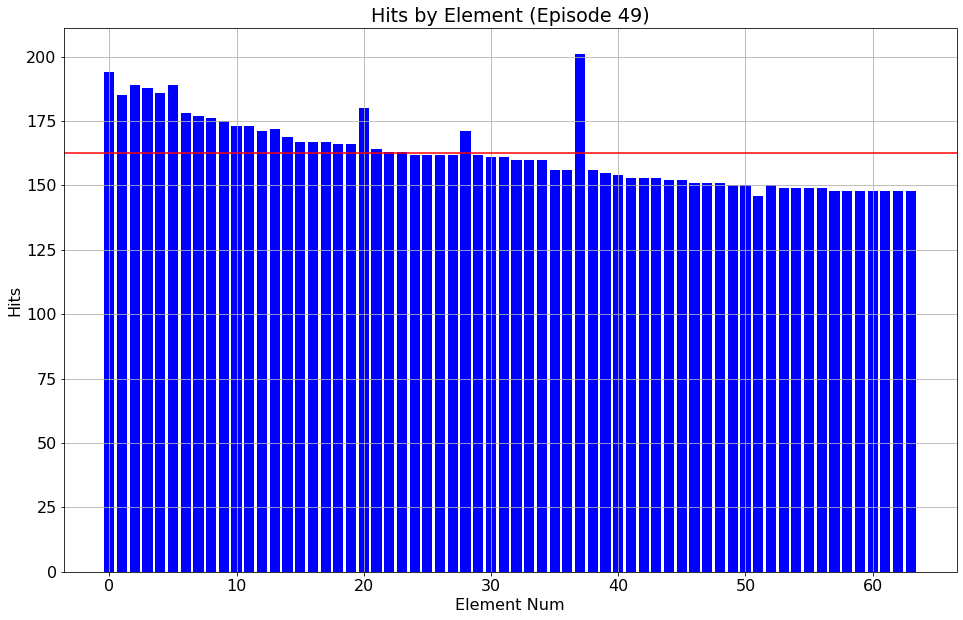
\includegraphics[width=\linewidth]{../figs/search_known/unperturbed/hits.png}
% \caption{}
\end{subfigure}
\medskip
\begin{subfigure}[t]{\subfigwidth\textwidth}
\centering
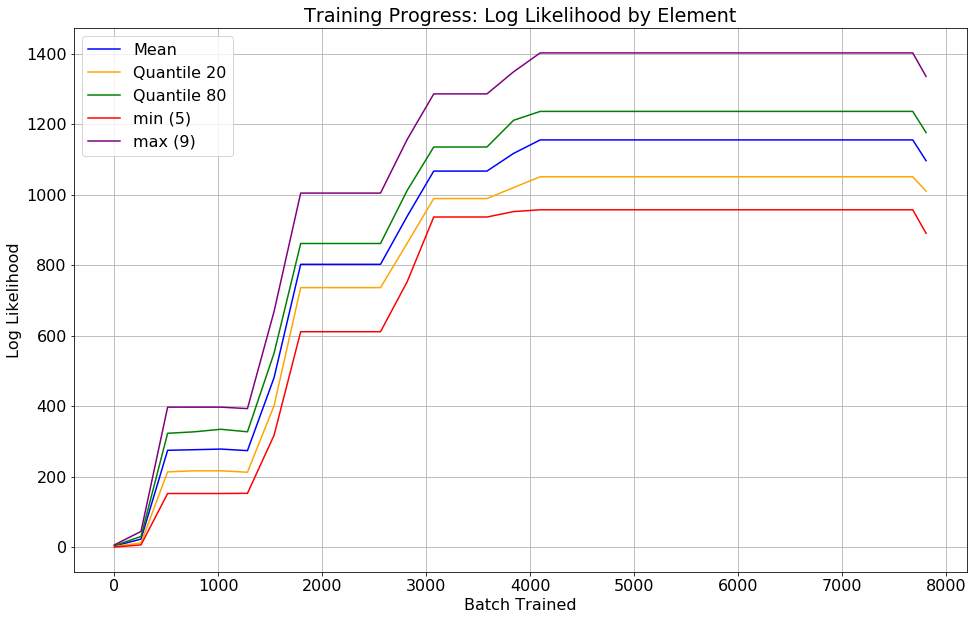
\includegraphics[width=\linewidth]{../figs/search_known/unperturbed/learning_curve_log_like.png}
% \caption{}
\end{subfigure}
\hfill
\begin{subfigure}[t]{\subfigwidth\textwidth}
\centering
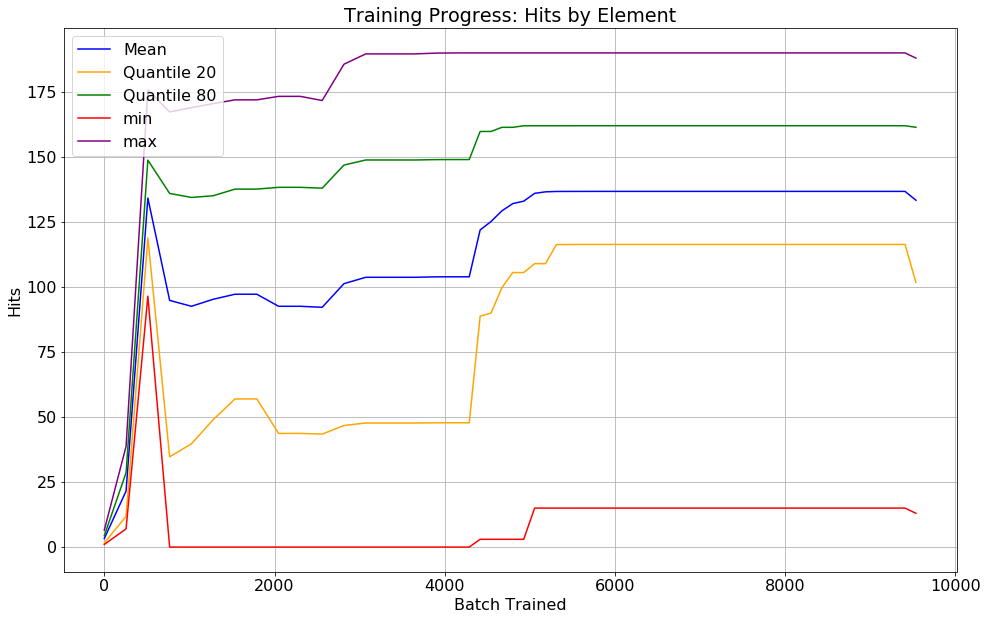
\includegraphics[width=\linewidth]{../figs/search_known/unperturbed/learning_curve_hits.png}
% \caption{}
\end{subfigure}
\caption{Training progress on 64 unperturbed orbital elements.}
\end{figure}

\begin{figure}[hbt!]
\begin{center}
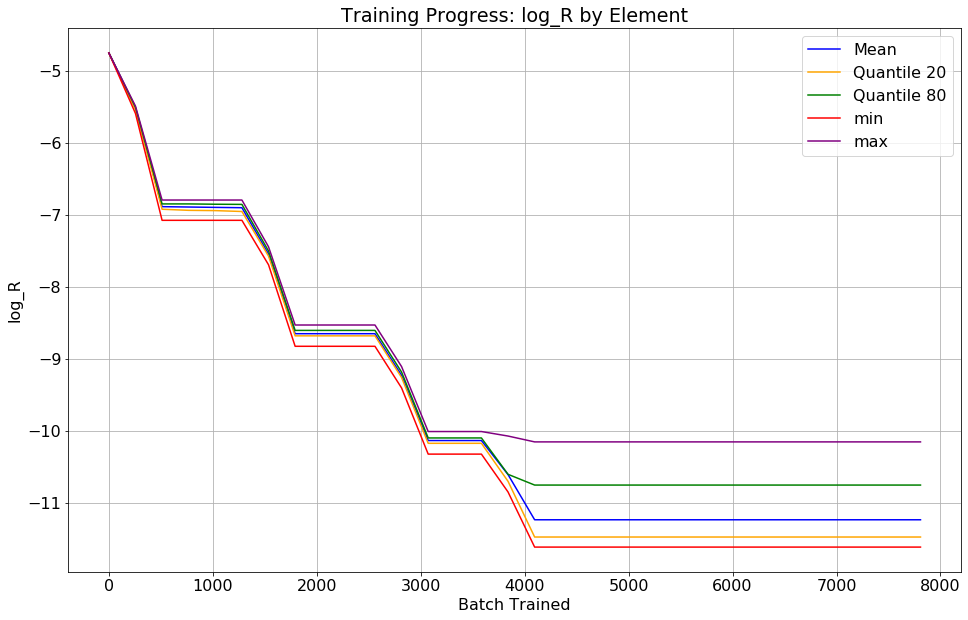
\includegraphics[width=1.0\textwidth]{../figs/search_known/unperturbed/learning_curve_log_R.png}
\caption{The resolution $R$ decreases monotonically when training the unperturbed elements.}
\end{center}
\end{figure}

We can see that the model is behaving as hoped.
It is gradually ratcheting the resolution parameter and scoring a high log likelihood as it does so.
It does this without getting deked and polluting the originally correct orbital elements.

The diagnostics presented above work equally well for any set of candidate orbital elements,
whether or not they are ostenisbly associated with a known asteroid.
In this case, we can further validate the results by comparing our fitted elements to the nearest asteroid
using the two metrics described in the previous section.

Here is a data frame comparing the recovered elements with the nearest asteroid 
\begin{figure}[h]
\begin{center}
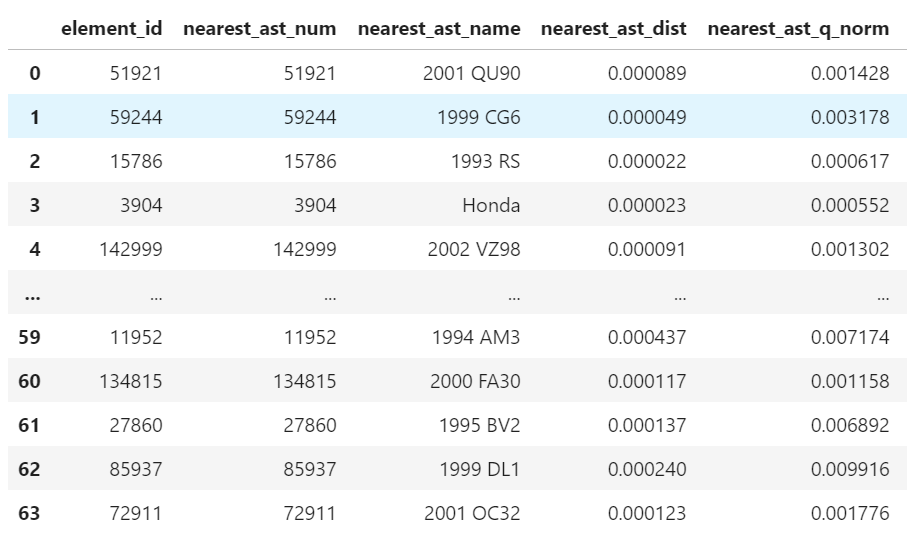
\includegraphics[width=1.0\textwidth]{../figs/search_known/unperturbed/nearest_ast_dataframe.png}
\caption{The nearest asteroid to the recovered elements initialized with unperturbed asteroid elements.}
\end{center}
\end{figure}
The simplest test is how many of 64 recovered elements have as their nearest asteroid the same asteroid used to initialize the elements.
The answer is 64: the fitting process ``tried'' to converge back to the right asteroid every time.
A more substantive question is how close did it come.  
Here are the geometric mean differences of two metrics:
\begin{itemize}
\item Distance in AU: 6.61E-6
\item Covariance Norm of elements: 2.00E-3
\end{itemize}
This is an excellent level of agreement.
The covariance norm is a good summary statistic, but may be hard to relate to astronomy.
The mean absolute error in the recovered $a$ is 4.3E-4 and in the recovered $e$ is 1.6E-4.

Here are two visualizations showing the distance in AU and covariance norm to the nearest (original) asteroid for all 64 candidate elements.
\begin{figure}[h]
\begin{center}
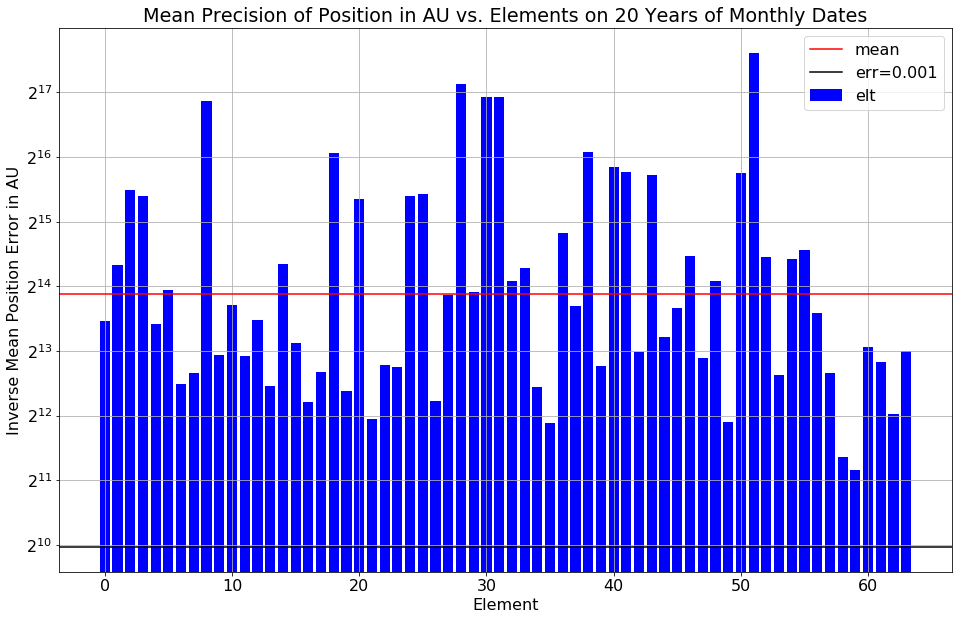
\includegraphics[width=1.0\textwidth]{../figs/search_known/unperturbed/near_ast_dist.png}
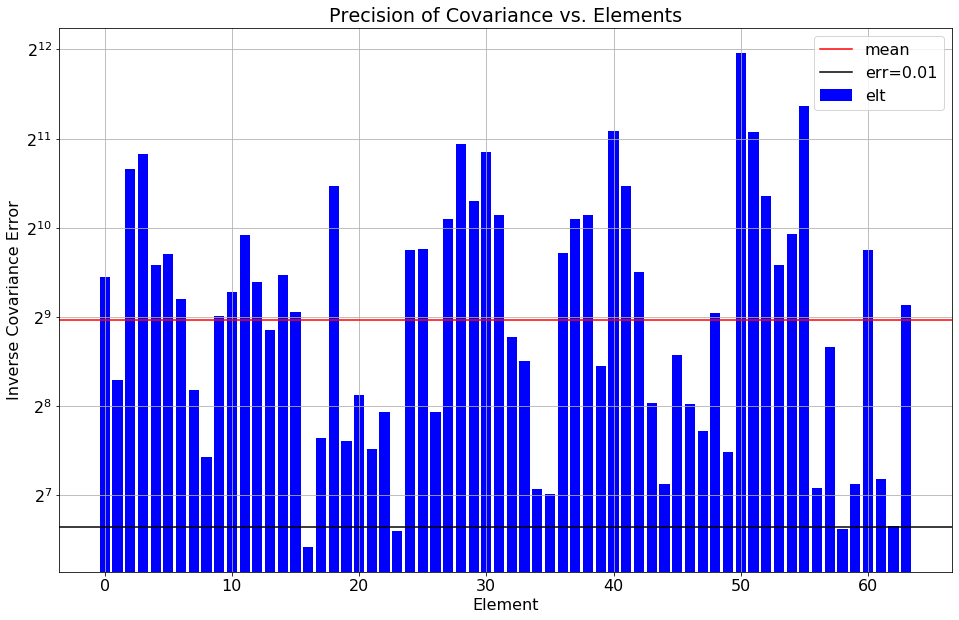
\includegraphics[width=1.0\textwidth]{../figs/search_known/unperturbed/near_ast_cov.png}
\caption{Two metrics comparing the recovered orbital elements to the true elements of the asteroid in question.\\
Both charts are plotted on a log scale with preicision (reciprocal of the error) on the $y$ axis.\\
The geometric mean error is shown in red: 6.61E-6 AU and 2.00E-3 on the covariance norm.}
\end{center}
\end{figure}
\clearpage

\section{Recovering the Perturbed Elements of Known Asteroids}
\label{section_results_known_ast_perturbed}

\subsection{Small Perturbation}
The next experiment is similar to the previous one.
This time we will apply a small perturbation to the orbital elements in our initial guess.
If the last experiment was like hitting a tee ball, this one may be likened to hitting a ball gently pitched by your little league coach in batting practice.
The elements are perturbed using the function \tty{perturb\_elts} in \tty{candidate\_elements.py}.
The perturbation adds normally distributed random noise with the specified standard deviation
to $\log(a)$, $\log(e)$, and the four angles $i$, $\Omega$, $\omega$ and $f$.
The small perturbation shifts $\log(a)$ by $0.01$, $\log(e)$ by $0.0025$, $i$ by $0.05$ degrees,
and the the other angles by $0.25$ degrees.
A random seed is used for reproducible results
The code to do this is
\begin{lstlisting}[style=CodeSnippet]
elts_pert= perturb_elts(elts_ast, sigma_a=0.01, sigma_e=0.0025, 
	sigma_inc_deg=0.05, sigma_f_deg=0.25, 
	sigma_Omega_deg=0.25, sigma_omega_deg=0.25,
	random_seed=42)
\end{lstlisting}
Last time we the summary statistic based on $\log(v)$ showed a very positive $t$ score.
This time the $t$ score has dropped to $+3.71$, and the model has zero hits before it begins training.
Even this small perturbation is enough that the model is going to have to work quite a bit to recover the elements.

Here is the text report after sieving:
\begin{lstlisting}[style=CodeSnippet]
Good elements (hits >= 5):  32.00
         \  log_like :  hits  :    R_sec : thresh_sec
Mean Good:   798.22  :  73.00 :    42.71 :  1013.88
Mean Bad :   151.47  :   0.16 :   246.08 :  2130.53
Min      :     1.33  :   0.00 :     3.53 :   233.61
Max      :  1226.84  : 163.00 :  1168.61 :  2400.00
Trained for 12096 batches over 189 epochs and 71 episodes (elapsed time 520 seconds).
\end{lstlisting}

Here are summary statistics for the run on the small perturbation of real asteroid elements:
\begin{itemize}
\item Successfully converged for 32 out of 64 candidate elements
\item Mean hits on converged elements: 73.00
\item Resolution on converged elements: 42.7 arc seconds
\item Distance in AU to nearest asteroid: 4.00E-4
\item Covariance Norm to nearest asteroid: 1.69E-2
\end{itemize}
These results are not as strong as on the unperturbed elements, but the method is still clearly working.
It's coverged on half of the candidate orbital elements.
The converged elements are fit well, average 73 hits at 43 arc seconds.
The distance to the nearest asteroid is 4.0E-4 AU, which is still very close and an excellent description of the orbit.

\begin{figure}[h]
\begin{subfigure}[t]{\subfigwidth\textwidth}
\centering
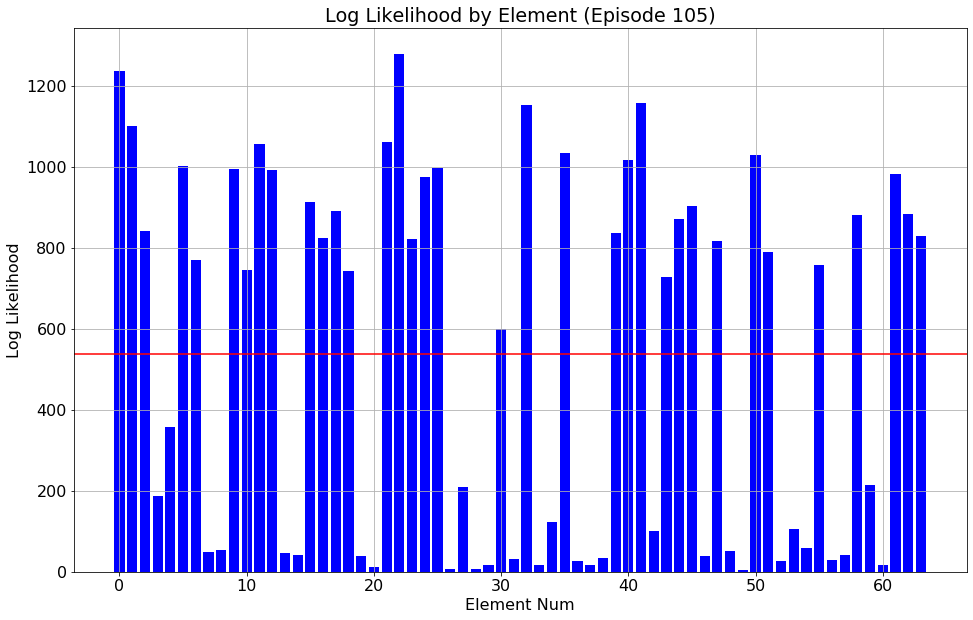
\includegraphics[width=\linewidth]{../figs/search_known/perturbed_small/log_like.png}
% \caption{}
\end{subfigure}
\hfill
\begin{subfigure}[t]{\subfigwidth\textwidth}
\centering
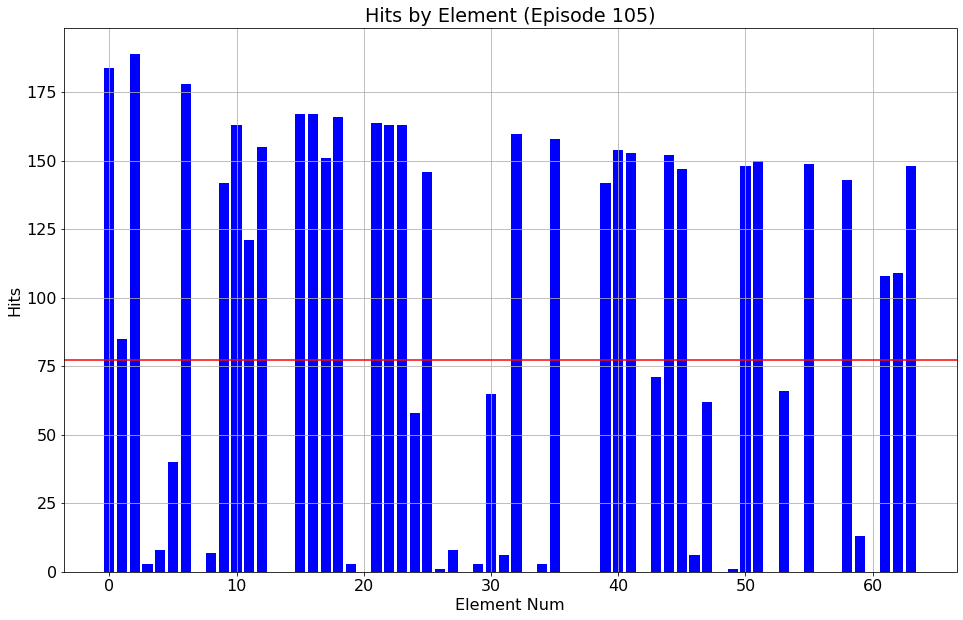
\includegraphics[width=\linewidth]{../figs/search_known/perturbed_small/hits.png}
% \caption{}
\end{subfigure}
\medskip
\begin{subfigure}[t]{\subfigwidth\textwidth}
\centering
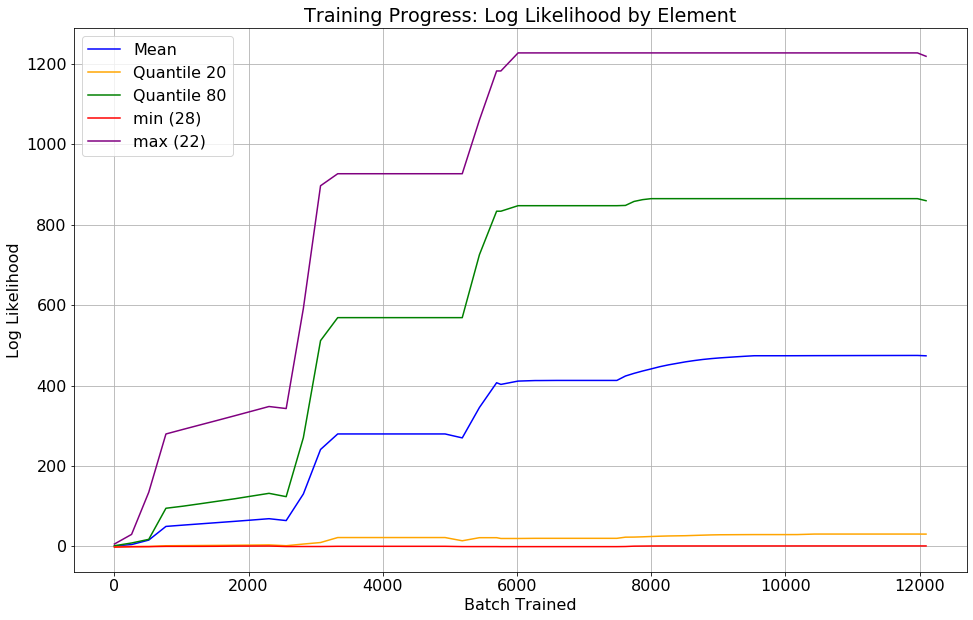
\includegraphics[width=\linewidth]{../figs/search_known/perturbed_small/learning_curve_log_like.png}
% \caption{}
\end{subfigure}
\hfill
\begin{subfigure}[t]{\subfigwidth\textwidth}
\centering
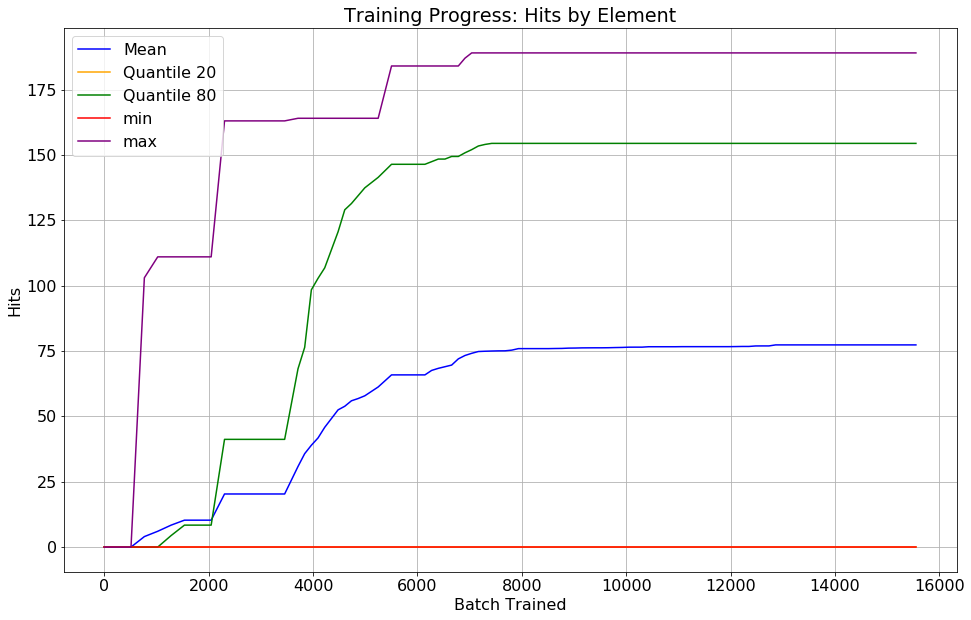
\includegraphics[width=\linewidth]{../figs/search_known/perturbed_small/learning_curve_hits.png}
% \caption{}
\end{subfigure}
\medskip
\begin{subfigure}[t]{\textwidth}
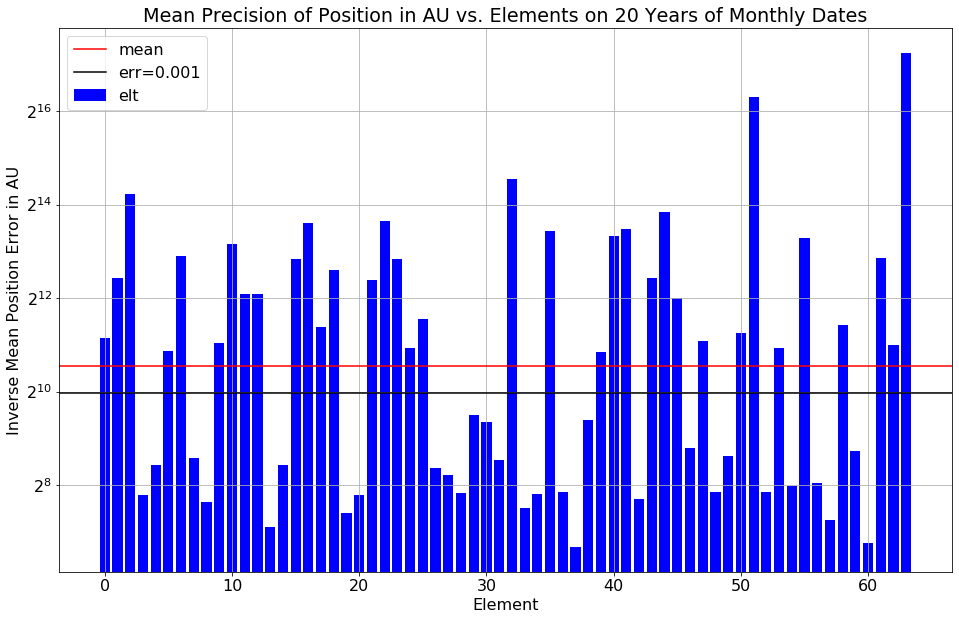
\includegraphics[width=1.0\textwidth]{../figs/search_known/perturbed_small/near_ast_dist.png}
\end{subfigure}
\caption{Training progress on 64 orbital elements initialized with small perturbations from real asteroids.\\
32 of the 64 candidate elements converge, averaging 73 hits each.}
\end{figure}
\clearpage

\subsection{Large Perturbation}
In our third test, we will again start with perturbed orbital elements.
But this time, we will apply a much larger perturbation.
This is a much harder task.  
To continue with the baseball analogy, it might be like batting in a high school game.
The perturbation size this time is 0.05 on $\log(a)$, $0.01$ on $\log(e)$, $0.25$ degrees on $i$, and $1.0$ degree on the other three angles.
While this might not sound like much at first, they are large perturbations.
In fact, they are so large they led me down a painful rabbit hole.
I repeatedly failed to recover the orbital elements of the original asteroids 
before I realized that the perturbations were large enough that in many cases, 
the nearest asteroid to the perturbed element was no longer the original asteroid!
The results started to make much more sense when I compared each fitted element to the nearest real asteroid,
regardless of whether this matched the original source of the elements before perturbation.

Here is the text report after sieving:
\begin{lstlisting}[style=CodeSnippet]
Good elements (hits >= 5):   9.00
         \  log_like :  hits  :    R_sec : thresh_sec
Mean Good:   950.21  :  87.33 :    26.00 :   801.43
Mean Bad :    42.19  :   0.11 :   252.31 :  2347.92
Min      :     8.83  :   0.00 :     2.92 :   341.62
Max      :  1351.26  : 163.00 :   742.89 :  2400.00
Trained for 13056 batches over 204 epochs and 76 episodes (elapsed time 547 seconds).
\end{lstlisting}

Here are summary statistics for the run on the small perturbation of real asteroid elements:
\begin{itemize}
\item Successfully converged for 9 out of 64 candidate elements
\item Mean hits on converged elements: 87.00
\item Resolution on converged elements: 26.0 arc seconds
\item Distance in AU to nearest asteroid: 4.11E-4
\item Covariance Norm to nearest asteroid: 3.18E-2
\end{itemize}
This time we've only converged on 9 of the 64 orbital elements.
But the encouraging news is that when we have converged, the fit is as good as it was before.
The average hits are 87 and the resolution is 26.0 arc seconds.
The distance to the nearest asteroid is comparable to the batch initialized with small perturbations, at 4.0E-4.
This is telling us something important: 
when the model starts from a good enough guess that it has a path in search space to the local maximum, it will converge to a good solution.
Starting from a poor initialization will reduce the probability of successful convergence, but it doesn't dilute the quality of the results.

\begin{figure}[h]
\begin{subfigure}[t]{\subfigwidth\textwidth}
\centering
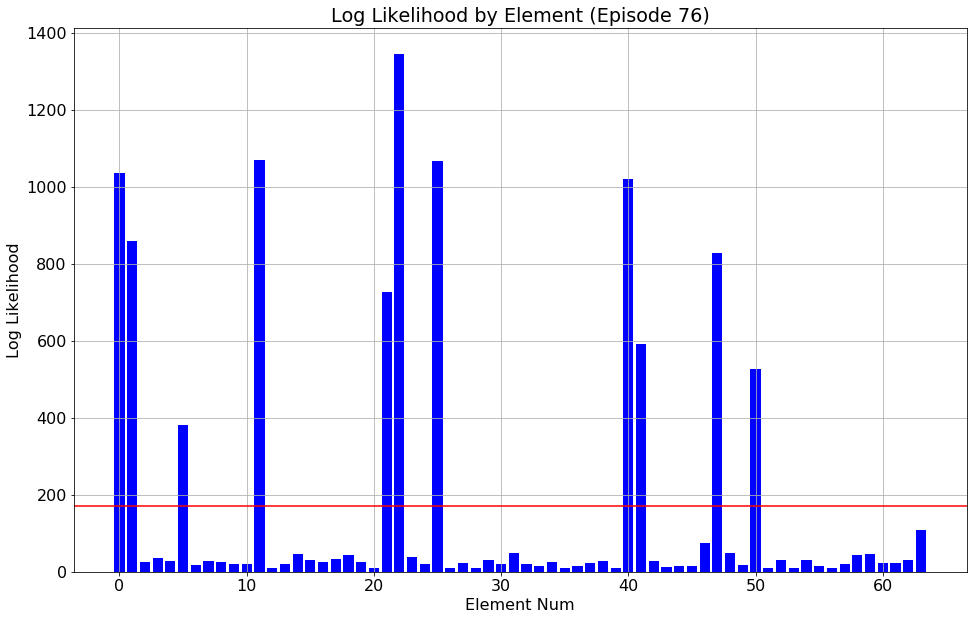
\includegraphics[width=\linewidth]{../figs/search_known/perturbed_large/log_like.png}
% \caption{}
\end{subfigure}
\hfill
\begin{subfigure}[t]{\subfigwidth\textwidth}
\centering
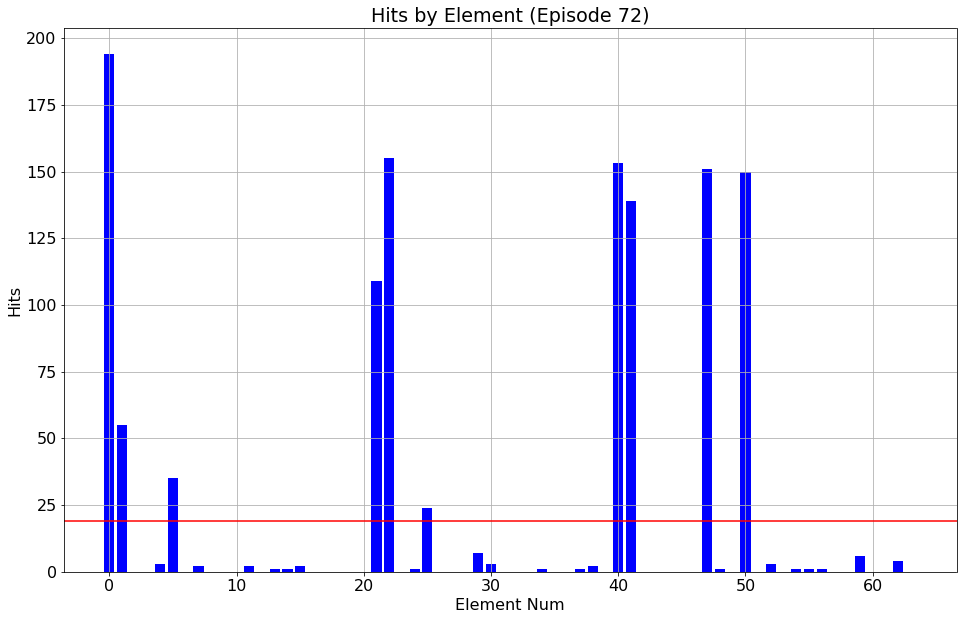
\includegraphics[width=\linewidth]{../figs/search_known/perturbed_large/hits.png}
% \caption{}
\end{subfigure}
\medskip
\begin{subfigure}[t]{\subfigwidth\textwidth}
\centering
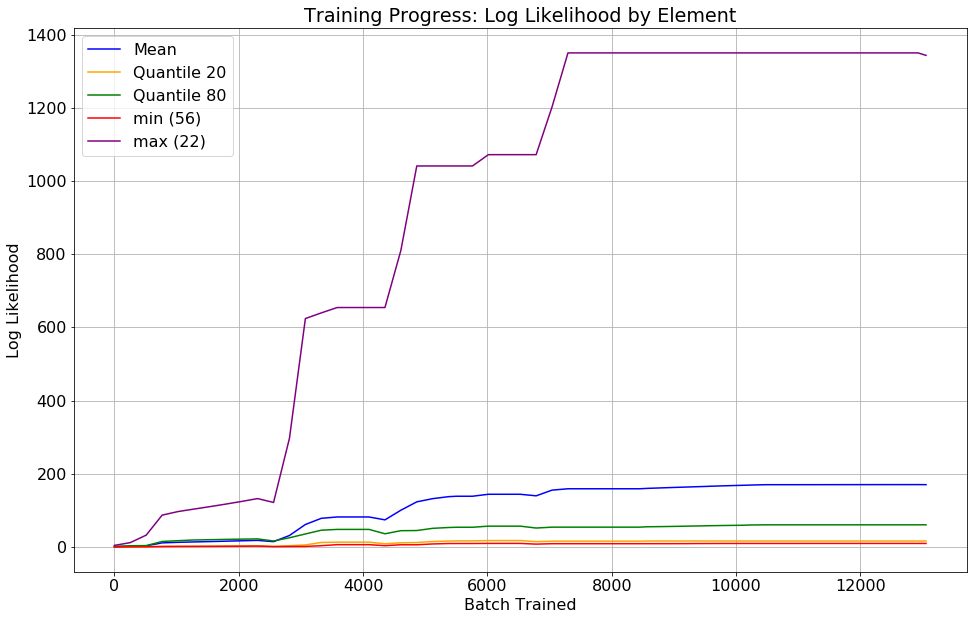
\includegraphics[width=\linewidth]{../figs/search_known/perturbed_large/learning_curve_log_like.png}
% \caption{}
\end{subfigure}
\hfill
\begin{subfigure}[t]{\subfigwidth\textwidth}
\centering
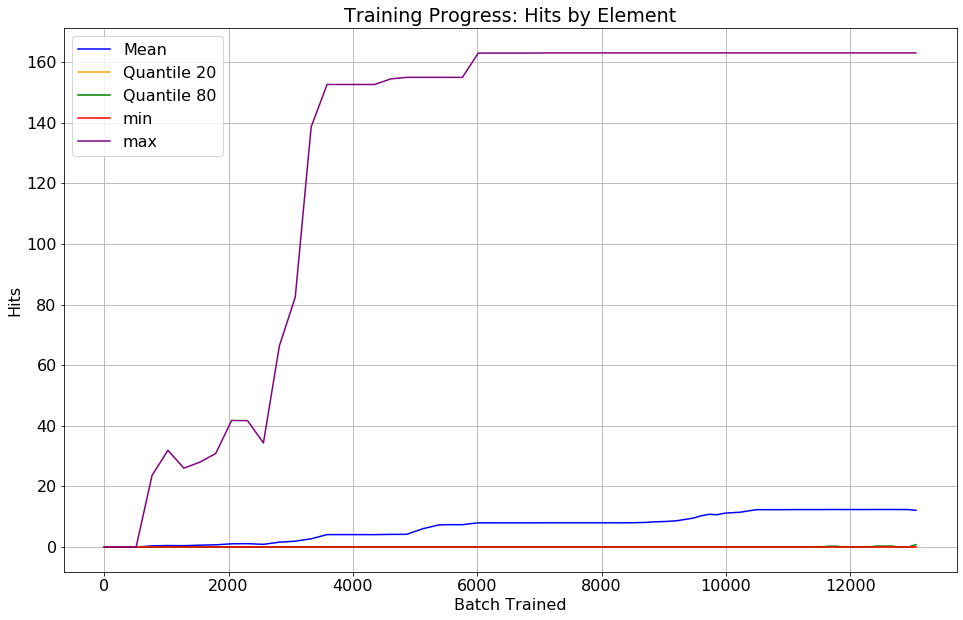
\includegraphics[width=\linewidth]{../figs/search_known/perturbed_large/learning_curve_hits.png}
% \caption{}
\end{subfigure}
\medskip
\begin{subfigure}[t]{\textwidth}
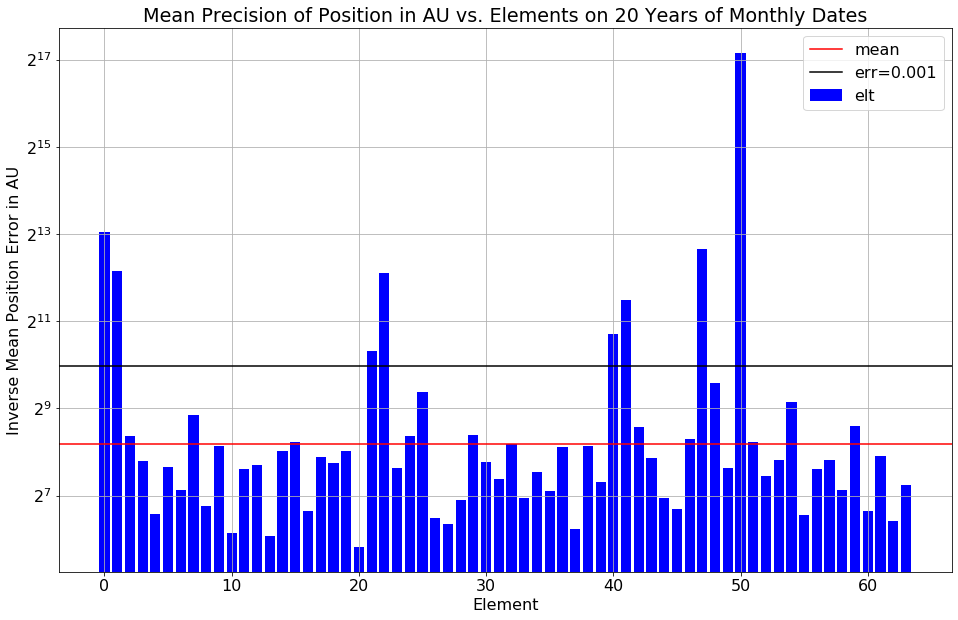
\includegraphics[width=1.0\textwidth]{../figs/search_known/perturbed_large/near_ast_dist.png}
\end{subfigure}
\caption{Training progress on 64 orbital elements initialized with large perturbations from real asteroids.\\
9 of the 64 elements converge, averaging 87 hits.}
\end{figure}
\clearpage

\section{Searching for Known Asteroids with Random Initializations}
\label{section_results_known_ast_random}
Our final test case before search for new asteroids is to attempt to recover asteroids in the known catalog, but without peeking at the answers.
I will now transition from small tests on a single batch 64 candidate elements to analyisis of the results of a large scale computational job.
The program \tty{asteroid\_search.py} can be run from the command line.
It searches against one of two subsets of the ZTF data set.
When run in ``known asteroids'' mode, the ZTF observations are filtered to include only the 3.69 m rows that are within 2.0 arc seconds of a known asteroid.
When run in ``unknown asteroids'' mode, it searches in the complement, those ZTF detections that are at least 2.0 arc seconds from a known asteroid.
The other arguments include the range of random seeds \tty{seed0} to \tty{seed1} and a stride to support parallelization.

This program was run on approximately 4096 random seeds against the known asteroids over the better part of a week.
Once a ZTF observation was associated with a set of candidate elements, it was subtracted from the data set so it would not be included in subsequent fits.
I filtered the results to those with at least 8 hits and a resolution of at most 20 arc seconds.
The results are reviewed in the Jupyter notebook \tty{19\_search\_known.ipynb}.
Since this was a search against known orbital elements, 
we can gauge the quality by measuring the distance of the recovered orbits to the nearest known asteroid.
Here are the summary statistics for the resulting fitted elements:
\begin{itemize}
\item 125 fitted orbital elements were found
\item they had 17.83 hits on average
\item the geometric mean resolution was 12.8 arc seconds
\item the geometric mean distance to the nearest asteroid was 2.7E-3 AU
\end{itemize}

\begin{figure}[h]
\begin{center}
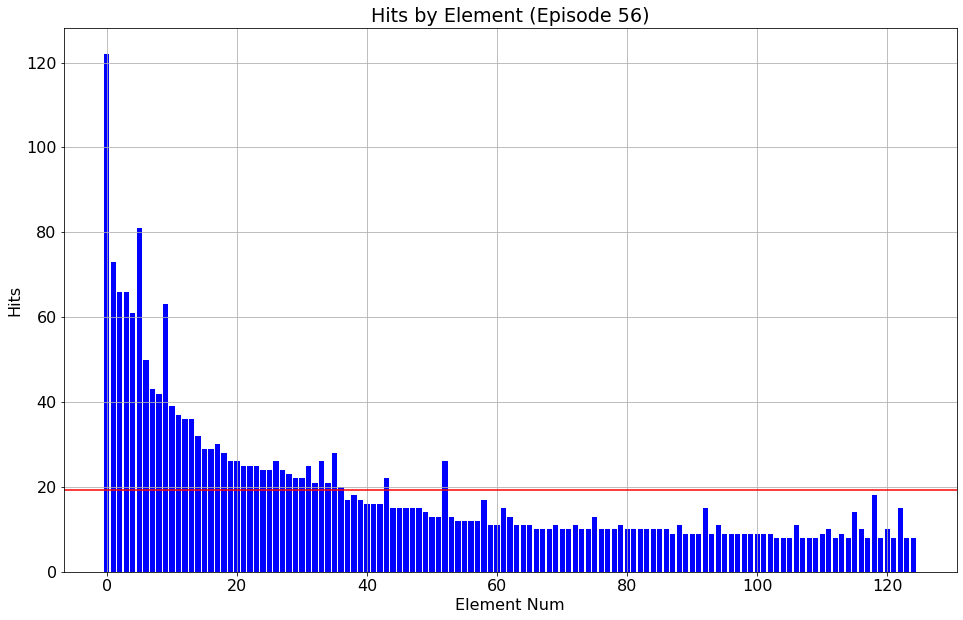
\includegraphics[width=0.70\textwidth]{../figs/search_known/random/hits.png}
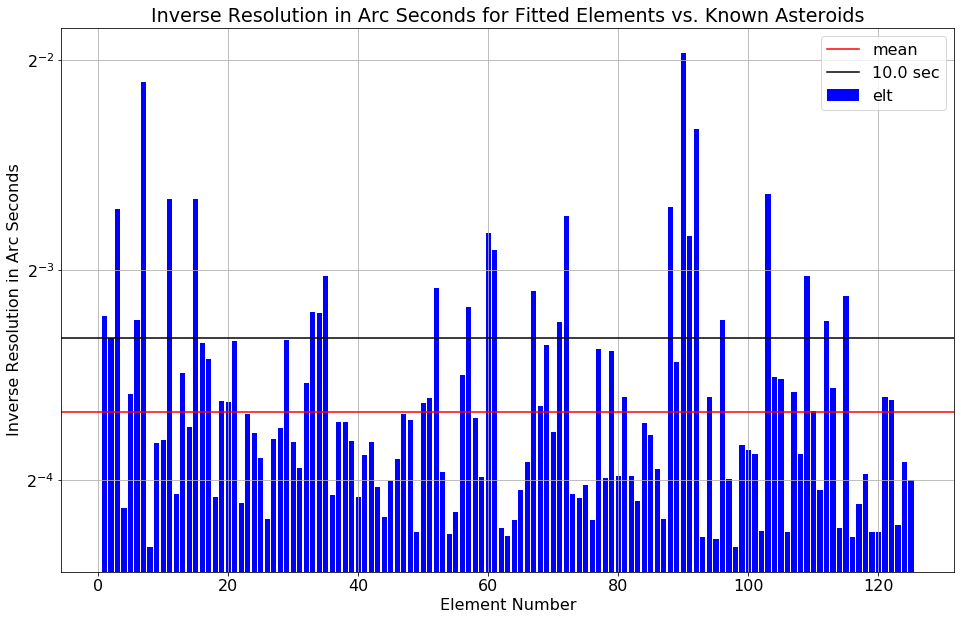
\includegraphics[width=0.70\textwidth]{../figs/search_known/random/resolution.png}
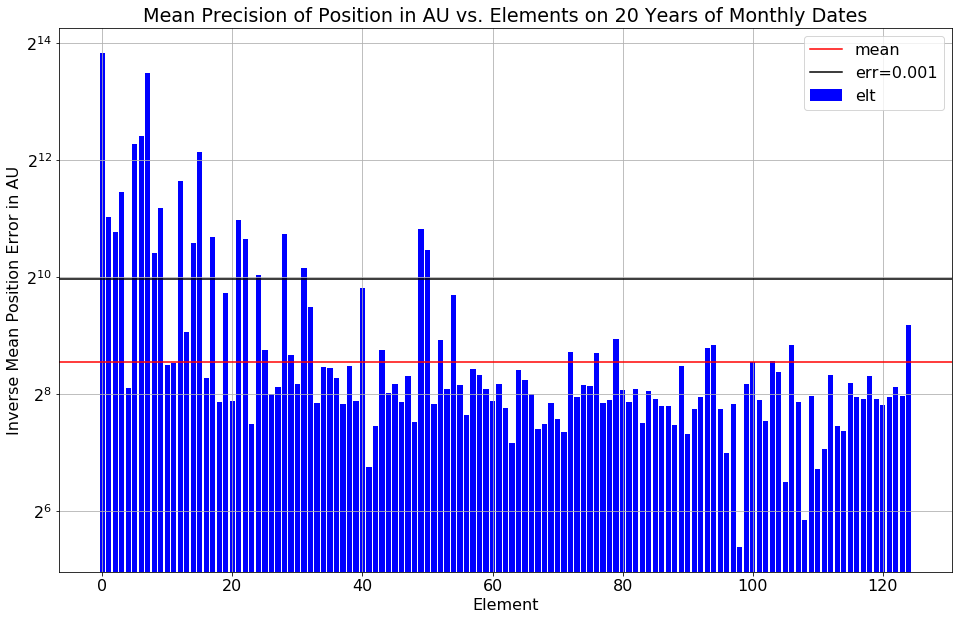
\includegraphics[width=0.70\textwidth]{../figs/search_known/random/near_ast_dist.png}
\caption{Recovered orbital elements of 125 known asteroids in the catalogue, starting from random initializations.}
\end{center}
\end{figure}
\clearpage
I thought these results were respectable but not great.
I will need to significantly improve the initializations to get a higher yield.
But I view this as a successful proof of concept that this technique can recover correct orbits of asteroids 
in the catalogue without peeking at the correct orbital elements.
I chart below the hits, resolution, and precision in AU vs. known orbital elements.

\section{Presenting 9 Previously Unknown Asteroids}
\label{section_results_unknown_ast}

\section{Conclusion}
\label{search_conclusion}

\section{Future Work}
\label{section_future_work}
